\section{Introduction}\label{sec:Introduction}

Here we present the results of the calorimetry tuning done for a sample of data and Monte Carlo spanning Run I and Run II of the LArIAT experiment. This calibration method is predicated on the Bethe-Block description of the mean rate of energy loss for various particle species. This is best represented by Figure \ref{fig:PDGEnergyLoss}, taken from the Particle Data Group \cite{PDG}.

\begin{figure}[htb]
\centering
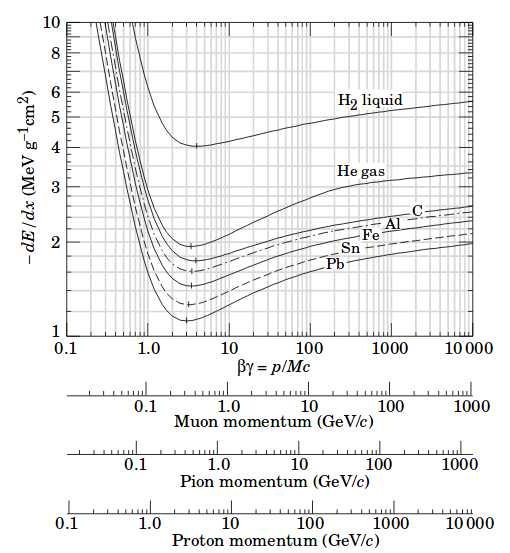
\includegraphics[width=0.50\textwidth]{images/PDGdEdX.png}
\caption{Mean energy loss in various materials over a range of particle momentums as produced in Reference \cite{PDG}.}
\label{fig:PDGEnergyLoss}
\end{figure}

Using the tables provided by the PDG for liquid argon (\cite{PDG-Argon}), we calculate the theoretical values for pions ($\pi$), muons ($\mu$), and protons ($p$) in the momentum range most relevant for LArIAT, shown in Figure \ref{fig:PDGEnergyLossArgon}.

\begin{figure}[htb]
\centering
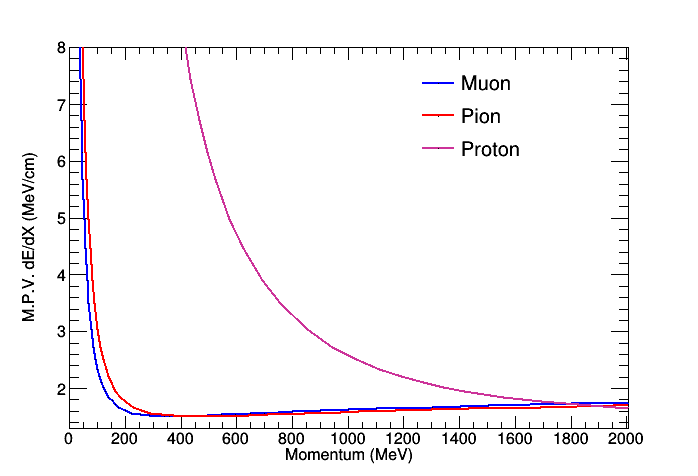
\includegraphics[width=0.50\textwidth]{images/dEdXvsMomentumTemplate}
\caption{Mean energy loss for pions, muons, and protons in liquid argon over the momentum range most relvant for LArIAT.}
\label{fig:PDGEnergyLossArgon}
\end{figure}

Using the predictions in Figure \ref{fig:PDGEnergyLossArgon}, allows us to tune the calorimetry constants used to convert the ADC to charge. The goal is to have the data and MC agree across the broad range of momentum. This tuning is done in addition to the wire-by-wire corrections (described in detail in \href{http://lartpc-docdb.fnal.gov:8080/cgi-bin/RetrieveFile?docid=1994&filename=investigation-uniformity-observed_v3.pdf&version=2}{doc-DB 1994}) and the usual lifetime corrections (described in detail in \href{http://lartpc-docdb.fnal.gov:8080/cgi-bin/ShowDocument?docid=1804}{docDB-1804}) which are used here and a more detailed treatment is left to their corresponding technical notes.

%%%%%%%%%%%%%%%%%%%%%%%%%%%%%%%%%%%%%%%%%%%%%%%%%%%%%%%%%%%
\subsection{Calibration Method Overview}\label{sec:MethodOverview}
%%%%%%%%%%%%%%%%%%%%%%%%%%%%%%%%%%%%%%%%%%%%%%%%%%%%%%%%%%%

In this section, we will describe the methodology we use to select our samples and tune the calorimetry constants. Details specific to any one sample will be described in Section  \ref{sec:EventSelection} and instead we will present the general method and how it is applied. 